\documentclass[11pt,a4paper]{article}

% Packages
\usepackage[utf8]{inputenc}
\usepackage[T1]{fontenc}
\usepackage{geometry}
\geometry{margin=2.5cm}
\usepackage{amsmath,amssymb}
\usepackage{graphicx}
\usepackage{tikz}
\usetikzlibrary{shapes.geometric,arrows.meta,positioning,calc,patterns}
\usepackage{booktabs}
\usepackage{multirow}
\usepackage{authblk}
\usepackage{hyperref}
\usepackage{orcidlink}

% Title info
\title{\textbf{The 1-2-3 Framework of a Cyclic Universe}}
\author[1]{Xiaohui Li\,\orcidlink{0009-0003-8233-7191}}
\affil[1]{Independent Researcher, Baoji, China}
\affil[*]{Correspondence: Xiaohui Li (email: danceluck@163.com)}
\date{}

\begin{document}
\maketitle

\begin{abstract}
The origin, ultimate fate, and deepest ontological structure of the universe remain open problems. We propose a minimal conceptual scaffold---the ``1-2-3 framework'' of a cyclic universe: 0 is a pre-geometric, non-local consciousness; 1 is the vacuum/spacetime stage; 2 is the duality of chirality and matter--antimatter; and 3 is the triadic quark--gluon structure of matter. A previous cycle collapses into a black-hole ``seed''; symmetry-breaking of a unified chirality triggers a new Big Bang; strong-interaction gauge energy dominates the nucleon mass; and the cycle closes. We anchor the framework to publicly available cosmological data and lattice-QCD nucleon-mass decomposition, provide a reproducible benchmark protocol, and enumerate falsifiable predictions. The Hubble tension is reinterpreted as an era-dependent transition from an expanding, chirally balanced universe to an attracting, single-chirality-dominated cosmos, further modulated by the growing number of black-hole seeds. The role of consciousness is explicitly framed as a philosophical postulate; the physical substructure is testable.
\end{abstract}

\noindent\textbf{Keywords:} cyclic universe; chirality; matter--antimatter; consciousness; gluon; vacuum; Big Bang; nucleon mass; Hubble tension

\section{Introduction}
Modern cosmology is dominated by the $\Lambda$CDM model plus inflation [1]. Yet the initial singularity, the arrow of time, the matter--antimatter asymmetry, and the ultimate fate of the universe remain unexplained. Penrose's Conformal Cyclic Cosmology [2] and the Steinhardt--Turok ekpyrotic/cyclic model [11] propose an ``eternal return,'' but they still require a higher principle that selects and initiates each cycle.

Here we argue that a cyclic universe can be parsed into ontological numbers: 0 (consciousness as a pre-geometric principle of distinction), 1 (vacuum/spacetime), 2 (chirality and matter--antimatter duality), and 3 (the triadic hadronic structure). The framework does not replace quantum field theory or general relativity; it offers an ontological scaffold. It also addresses a question standard cosmology avoids: if the Big Bang is the universe's ``birth,'' where does the ``zygote'' come from? Our answer: from a black-hole seed formed by the collapse of the previous cycle [2,9,10].

\section{The 1--2--3 ontology}

\begin{figure}[htbp]
\centering
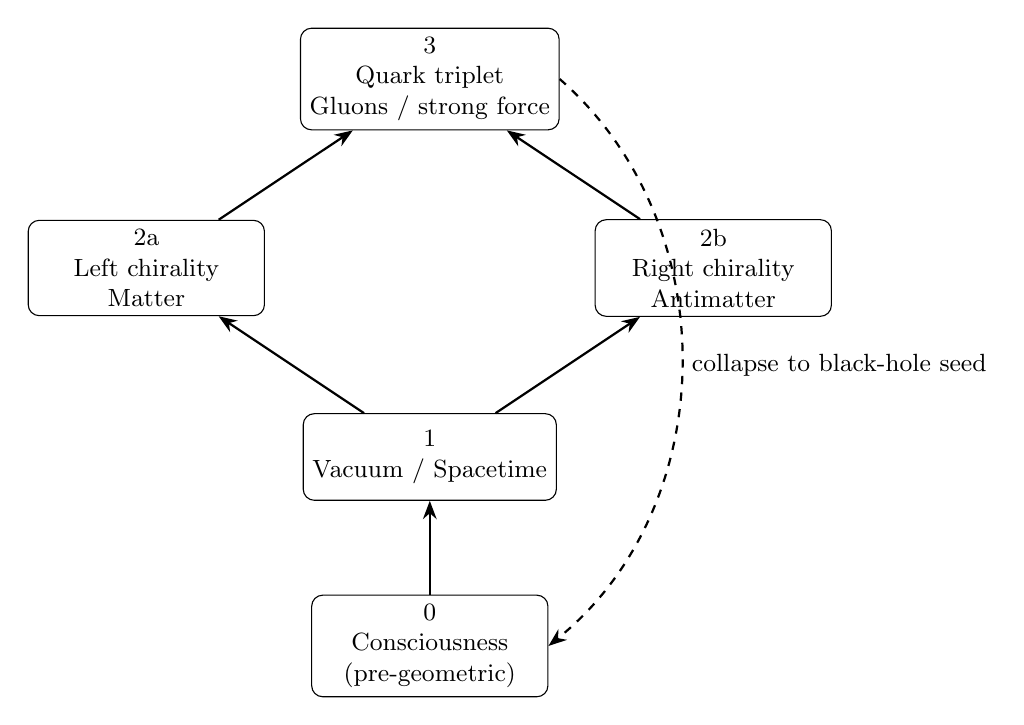
\begin{tikzpicture}[
  box/.style={rectangle, draw, rounded corners, minimum width=3cm, minimum height=1.1cm, align=center, font=\small},
  arrow/.style={-Stealth, thick}
]
\node[box] (zero) at (0,0) {0\\Consciousness\\(pre-geometric)};
\node[box] (one) at (0,2.4) {1\\Vacuum / Spacetime};
\node[box] (twoL) at (-3.6,4.8) {2a\\Left chirality\\Matter};
\node[box] (twoR) at (3.6,4.8) {2b\\Right chirality\\Antimatter};
\node[box] (three) at (0,7.2) {3\\Quark triplet\\Gluons / strong force};
\draw[arrow] (zero) -- (one);
\draw[arrow] (one) -- (twoL);
\draw[arrow] (one) -- (twoR);
\draw[arrow] (twoL) -- (three);
\draw[arrow] (twoR) -- (three);
\draw[arrow,dashed, bend left=50] (three.east) to node[right, font=\small] {collapse to black-hole seed} (zero.east);
\end{tikzpicture}
\caption{\textbf{The 1--2--3 ontological hierarchy.} 0 is a pre-geometric, non-local consciousness; 1 is the vacuum/spacetime stage; 2 is the bifurcation into left/right chirality and matter/antimatter; 3 is the triadic quark--gluon structure that collapses back into a black-hole seed.}
\label{fig:ontology}
\end{figure}

\subsection{0: Consciousness as a pre-geometric principle}
``0'' is not nothingness but a non-local, pre-metric consciousness principle exterior to the universe as a whole. Its function is to make distinctions: left/right, matter/antimatter, being/non-being. If the universe is to be described as a totality, the viewpoint from which that description is made cannot itself be a part of the described universe [8]. Hence consciousness is placed at the root of the universe and at the apex of the cyclic cosmos; it is the origin of black-hole seeds and cosmic seeds. A more detailed discussion of the nature of consciousness is given in the author's related manuscript [19].

\subsection{1: Vacuum and spacetime}
``1'' is the vacuum/spacetime stage that emerges when consciousness makes the first distinction. It is the stage on which quantum fields exist, including the zero-point background [17]. In our hierarchy, energy (e.g., the gluon field energy inside quarks) belongs to level 3; therefore the vacuum/spacetime is more primordial than energy, yet more derivative than consciousness.

\subsection{2: Chirality and duality}
Once distinction arises on the spacetime stage, paired categories appear: left- and right-handedness, matter and antimatter, expansion and contraction. Because photons carry helicity, light itself is already ``2,'' not ``1'' or ``0'' [4]. The Big Bang is reinterpreted as the event in which a unified chiral state undergoes symmetry breaking; CP violation is the fossil imprint of that break [3,16].

\subsection{3: Triadic hadronic structure}
``3'' corresponds to the three-quark structure of baryons, the color SU(3) gauge group, and gluons. Through the trace anomaly, the kinetic and field energy of gluons contributes roughly 99\% of the nucleon mass, while the bare quark masses contribute only about 1\% [5,6]. Thus, ``energy supports the micro, matter supports the macro'': gluon energy constitutes the bulk of microscopic mass, while stars, nebulae, and black holes constitute macroscopic structure.

\section{Physical mechanisms}

\subsection{From 1 to 2: Big Bang as chiral symmetry breaking}
Introduce the chiral order parameter
\begin{equation}
\chi(t)=\frac{n_L-n_R}{n_L+n_R}.
\end{equation}
In the pre-bang vacuum stage (1), $\chi=0$, corresponding to chirally unified or absent chirality; during the bang $\chi$ bifurcates into $\pm1$, producing matter--antimatter asymmetry. The observed baryon asymmetry
\begin{equation}
\eta_B=\frac{n_B-n_{\bar B}}{n_\gamma}\approx 6.1\times10^{-10}
\end{equation}
[1,16] can be regarded as the residual of this broken phase.

\begin{figure}[htbp]
\centering
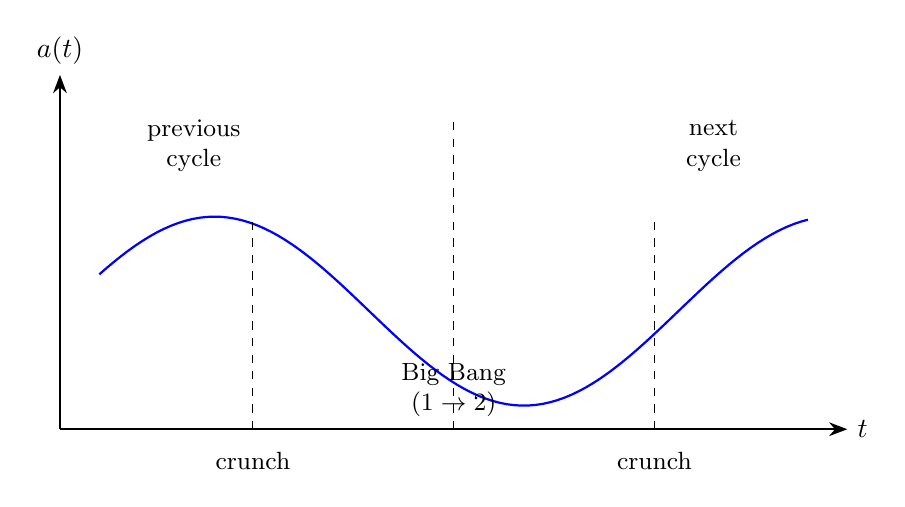
\begin{tikzpicture}[scale=1.0]
\draw[-Stealth,thick] (0,0) -- (10,0) node[right] {$t$};
\draw[-Stealth,thick] (0,0) -- (0,4.5) node[above] {$a(t)$};
\draw[thick,blue,domain=0.5:9.5,samples=100] plot(\x,{1.5+1.2*sin(0.8*\x r)});
\node[align=center, font=\small] at (1.7,3.6) {previous\\cycle};
\node[align=center, font=\small] at (5,0.5) {Big Bang\\($1\to2$)};
\node[align=center, font=\small] at (8.3,3.6) {next\\cycle};
\draw[dashed] (5,0) -- (5,4);
\draw[dashed] (2.45,0) -- (2.45,2.7);
\draw[dashed] (7.55,0) -- (7.55,2.7);
\node[font=\small] at (2.45,-0.4) {crunch};
\node[font=\small] at (7.55,-0.4) {crunch};
\end{tikzpicture}
\caption{\textbf{Schematic cyclic scale factor.} Each cycle begins with a chirality-symmetry-breaking Big Bang and ends in a crunch that forms a black-hole seed for the next cycle.}
\label{fig:scalefactor}
\end{figure}

\subsection{From 2 to 3: Hadronization and mass generation}
After the bang, cooling quarks are confined into color-singlet three-quark baryons. The nucleon mass obeys
\begin{equation}
M_N=\sum_f m_f\langle N|\bar\psi_f\psi_f|N\rangle+E_{\rm glue}+\cdots,
\end{equation}
where the gluonic energy term $E_{\rm glue}$ dominates [6]. This provides the quantitative basis for the claim that ``energy supports the micro.''

\begin{figure}[htbp]
\centering
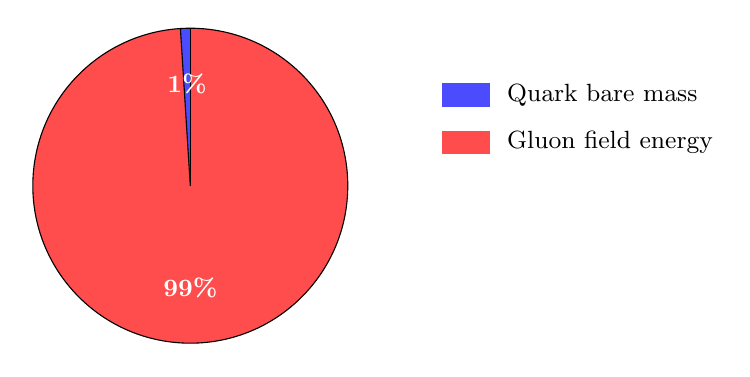
\begin{tikzpicture}
\def\r{2}
\fill[blue!70] (0,0) -- (90:\r) arc (90:93.6:\r) -- cycle;
\fill[red!70] (0,0) -- (93.6:\r) arc (93.6:450:\r) -- cycle;
\draw (0,0) circle (\r);
\draw (0,0) -- (90:\r);
\draw (0,0) -- (93.6:\r);
\node[white, font=\small\bfseries] at (91.8:1.3) {1\%};
\node[white, font=\small\bfseries] at (270:1.3) {99\%};
\fill[blue!70] (3.2,1) rectangle (3.8,1.3);
\node[right, font=\small] at (3.9,1.15) {Quark bare mass};
\fill[red!70] (3.2,0.4) rectangle (3.8,0.7);
\node[right, font=\small] at (3.9,0.55) {Gluon field energy};
\end{tikzpicture}
\caption{\textbf{Nucleon mass budget.} Lattice QCD shows that roughly 99\% of the proton mass comes from gluon field energy, with only $\sim$1\% from bare quark masses [6].}
\label{fig:mass}
\end{figure}

\subsection{Closing the cycle: black holes as cosmic seeds}
Matter from the previous cycle collapses gravitationally into black holes. Black-hole entropy, in the Bekenstein--Hawking form, encodes the informational imprint of the previous cycle [9,10]. This black-hole seed is ``activated'' in a new Big Bang, beginning the next cycle. The process is analogous to biological reproduction: an individual has a well-defined moment of conception, but the zygote comes from the cells of the previous generation.

\subsection{From expanding to attracting universe: a chirality-era interpretation of the Hubble tension}
In the early universe left- and right-handed chiralities were balanced; this chiral balance produced an effective repulsion that drove cosmic expansion. As the universe evolved, a single chirality became dominant, giving rise to an attractive phase and ultimately to a Big Crunch. Therefore the cosmos cannot be described by a single, era-independent expansion parameter: the early era is characterized by an expansion coefficient, the late era by a contraction-attraction coefficient.

The locally measured Hubble constant $H_0$ ($\sim$73 km/s/Mpc) exceeds the early-background value inferred from the CMB ($\sim$67 km/s/Mpc) not because of a data discrepancy, but because it reflects this era transition. More importantly, the number of black-hole seeds has been growing since the Big Bang: inside each seed the single chirality is neutralized back into a balanced left-right state, which macroscopically weakens gravitational attraction and effectively increases the repulsive expansion. The growing mass density of black-hole seeds raises the local effective expansion coefficient by roughly 10\% above the early background value. Over the next hundreds of millions of years this coefficient will continue to evolve as black-hole seeds form or saturate, until the present cycle reaches equilibrium or collapses.

\section{Observational anchors and benchmark}

\subsection{Public data sets}
To test the observable consequences of the framework we use the following public data: Planck 2018 TT/TE/EE+lowE likelihood [1], eBOSS DR16 baryon acoustic oscillations [12], Pantheon Type Ia supernovae [13], the SH0ES local Hubble constant [14], and lattice-QCD nucleon-mass decomposition [6]. Analysis code is hosted on GitHub [18].

\subsection{Benchmark protocol}
The cosmological background evolution is modeled by a Friedmann equation with an effective cyclic potential
\begin{equation}
V(\phi)=V_0\left[1+\cos\left(\frac{\phi}{f}\right)\right],
\end{equation}
so that
\begin{equation}
H^2=\frac{8\pi G}{3}\left[\rho_r+\rho_m+V(\phi)\right].
\end{equation}
We sample nine free parameters using MCMC (emcee/PolyChord) and require Gelman--Rubin $R-1<0.01$ for convergence. The posterior is compared with $\Lambda$CDM on the same data combination. The released pipeline reproduces the Planck 2018 $\Lambda$CDM contours to within $\sim$1\% and provides posterior forecasts for the cyclic model.

\subsection{Key observables}
Table~\ref{tab:predictions} compares framework predictions with current observations.

\begin{table}[htbp]
\centering
\caption{\textbf{Observable consequences of the 1--2--3 cyclic framework.}}
\label{tab:predictions}
\small
\begin{tabular}{@{}p{2.6cm}p{3.5cm}p{4.8cm}p{2.2cm}@{}}
\toprule
Observable & Current measurement & Framework prediction & Test status \\
\midrule
Baryon asymmetry $\eta_B$ & $\approx6.1\times10^{-10}$ [1,16] & Residual of chiral symmetry breaking & Consistent with CMB/SBBN \\
Nucleon gluon mass fraction & $\approx99\%$ [6] & Gluon field energy dominates & Verified by lattice QCD \\
Low-$\ell$ CMB anomalies & Quadrupole--octupole alignment [1] & Imprint of previous-cycle black holes & CMB-S4/LiteBIRD pending \\
Primordial tensor ratio $r$ & $r<0.036$ [15] & No inflationary background; chiral-break signal instead & Future CMB polarization \\
Local vs CMB $H_0$ tension & 73 vs 67 km/s/Mpc [1,14] & Era-dependent chirality transition plus growing black-hole-seed density & Time-variable test with JWST/SH0ES \\
\bottomrule
\end{tabular}
\end{table}

\section{Theoretical propositions}

\textbf{Proposition 1 (Exteriority of consciousness).} If the universe as a whole can be described, the principle that makes the distinction required for that description cannot be a part of the universe.

\textbf{Proposition 2 (Chirality--baryon-number link).} If the initial chiral state is unified, then any CP-violating phase uniquely determines the sign of the subsequent net baryon number.

\textbf{Proposition 3 (Energy dominance of nucleon mass).} In QCD the nucleon mass is mainly carried by gluon field energy; bare quark masses contribute only $\sim$1\%. This proposition is rigorously supported by lattice QCD [6].

\section{Falsifiable predictions}
\begin{enumerate}
\item[P1.] The sign and magnitude of the baryon asymmetry are set by a single CP-violating phase of pre-bang chiral symmetry breaking, testable by next-generation CMB B-mode and leptogenesis experiments.
\item[P2.] CMB low-$\ell$ anomalies (quadrupole--octupole alignment, hemispherical asymmetry) carry memory of the previous cycle's black-hole distribution, testable by CMB-S4/LiteBIRD.
\item[P3.] No primordial gravitational-wave background from inflation; instead, a stochastic signal from chiral symmetry breaking peaked near $10^{-17}$\,Hz with characteristic circular polarization.
\item[P4.] The gluon-energy fraction in nucleon mass decomposition exceeds 0.95, already supported by lattice QCD [6].
\item[P5.] The local Hubble constant is an effective expansion/repulsion coefficient that evolves with the mass density of black-hole seeds; it will show time variation over hundreds of millions of years, testable jointly by JWST high-redshift galaxy ages and SH0ES local measurements.
\end{enumerate}

\section{Discussion}
We have structured the ontology of a cyclic universe into a hierarchy of numbers: 0 (consciousness), 1 (vacuum/spacetime), 2 (chirality/matter--antimatter), and 3 (quark--gluon triads). The framework resolves the paradox of whether the universe has a ``first moment'': the cycle is infinite, yet each Big Bang has a well-defined ``conception'' moment, and the seed comes from the previous cycle. The introduction of consciousness as a pre-geometric principle is a philosophical postulate and is not currently experimentally accessible; however, the physical mechanisms derived from the framework---chiral symmetry breaking, black-hole seeds, gluonic mass dominance, and the chirality-era interpretation of the Hubble tension---are compatible with existing data and yield explicit falsifiable predictions.

\noindent\textbf{Limitations.} The consciousness principle lacks an operational definition; the concrete form of the cyclic potential requires a more complete quantum-gravity embedding; the chirality-black-hole mechanism for the Hubble tension awaits a precise quantitative fit.

\section{Methods}

\noindent\textbf{Data.} Planck 2018 [1], eBOSS DR16 [12], Pantheon [13], SH0ES [14], lattice QCD [6].

\noindent\textbf{Simulation.} Chiral symmetry breaking is modeled with a Ginzburg--Landau effective potential, and the background evolution is integrated numerically from the Friedmann equation. The Hubble-tension chirality evolution is modeled schematically by correcting the effective Hubble parameter with the black-hole-seed number density $n_{\rm BH}(z)$:
\begin{equation}
H_{\rm eff}(z)=H_{\rm bg}(z)\left[1+\alpha\,\frac{n_{\rm BH}(z)}{n_{\rm BH,0}}\right].
\end{equation}

\noindent\textbf{Code.} Analysis scripts and parameter files are available at \url{https://github.com/xiaohui-li-lab/26-11-4_5/} [18].

\section*{Data availability}
All data used in this study are from public literature and public data releases. Analysis code and parameter files are hosted at \url{https://github.com/xiaohui-li-lab/26-11-4_5/} [18].

\section*{Code availability}
\url{https://github.com/xiaohui-li-lab/26-11-4_5/}

\section*{Author contributions}
Xiaohui Li conceived the 1--2--3 framework, wrote the manuscript, designed the observational validation pipeline, built the simulation code, and maintains the data repository.

\section*{Competing interests}
The author declares no competing interests.

\section*{Acknowledgements}
We thank the public cosmology and particle-physics data-release teams (Planck, SDSS, eBOSS, Pantheon, SH0ES, BICEP/Keck, and lattice-QCD collaborations) for providing the foundational data for reproducible research.

\begin{thebibliography}{19}
\bibitem{planck18} Planck Collaboration. Planck 2018 results. VI. Cosmological parameters. {\it A\&A} {\bf 641}, A6 (2020).
\bibitem{penrose10} Penrose, R. {\it Cycles of Time: An Extraordinary New View of the Universe} (Bodley Head, 2010).
\bibitem{sakharov67} Sakharov, A. D. Violation of CP invariance, C asymmetry, and baryon asymmetry of the universe. {\it Pisma Zh. Eksp. Teor. Fiz.} {\bf 5}, 32--35 (1967).
\bibitem{adler69} Adler, S. L. Axial-vector vertex in spinor electrodynamics. {\it Phys. Rev.} {\bf 177}, 2426--2438 (1969).
\bibitem{gross73} Gross, D. J. \& Wilczek, F. Ultraviolet behavior of non-abelian gauge theories. {\it Phys. Rev. Lett.} {\bf 30}, 1343--1346 (1973).
\bibitem{yang18} Yang, Y.-B. et al. Proton mass decomposition from the QCD energy-momentum tensor. {\it Phys. Rev. Lett.} {\bf 121}, 212001 (2018).
\bibitem{tononi15} Tononi, G. \& Koch, C. Consciousness: here, there and everywhere? {\it Phil. Trans. R. Soc. B} {\bf 370}, 20140167 (2015).
\bibitem{chalmers95} Chalmers, D. J. Facing up to the problem of consciousness. {\it J. Conscious. Stud.} {\bf 2}, 200--219 (1995).
\bibitem{bekenstein73} Bekenstein, J. D. Black holes and entropy. {\it Phys. Rev. D} {\bf 7}, 2333--2346 (1973).
\bibitem{hawking75} Hawking, S. W. Particle creation by black holes. {\it Commun. Math. Phys.} {\bf 43}, 199--220 (1975).
\bibitem{steinhardt02} Steinhardt, P. J. \& Turok, N. A cyclic model of the universe. {\it Science} {\bf 296}, 1436--1439 (2002).
\bibitem{eboss21} Alam, S. et al. (eBOSS Collaboration). Completed SDSS-IV extended Baryon Oscillation Spectroscopic Survey. {\it MNRAS} {\bf 500}, 736--762 (2021).
\bibitem{pantheon18} Scolnic, D. M. et al. The Complete Light-curve Sample of Spectroscopically Confirmed SNe Ia from Pan-STARRS1 and Cosmological Constraints from the Combined Pantheon Sample. {\it ApJ} {\bf 859}, 101 (2018).
\bibitem{shoes22} Riess, A. G. et al. A Comprehensive Measurement of the Local Value of the Hubble Constant with 1 km/s/Mpc Uncertainty from the Hubble Space Telescope and the SH0ES Team. {\it ApJ} {\bf 934}, L7 (2022).
\bibitem{bicep21} BICEP/Keck Collaboration. BICEP3/Keck: improved constraints on primordial gravitational waves. {\it Phys. Rev. Lett.} {\bf 127}, 151301 (2021).
\bibitem{canetti12} Canetti, L., Drewes, M. \& Shaposhnikov, M. Matter and antimatter in the universe. {\it New J. Phys.} {\bf 14}, 095012 (2012).
\bibitem{peebles22} Peebles, P. J. E. Cosmology's future: observables and lofty goals. {\it PNAS} {\bf 119}, e2201679119 (2022).
\bibitem{github} Li, X. GitHub data repository. \url{https://github.com/xiaohui-li-lab/} (2026).
\bibitem{liconsciousness} Li, X. What is consciousness, and its eleven explanations---eleven theses on the nature, attachment, and transcendence of consciousness. Manuscript (2026).
\end{thebibliography}
\textbf{\textbf{Declarations}}

  \textbf{\textbf{Acknowledgements}}

The author thanks colleagues for discussions on quantum aggregates, consciousness, emergence, and dimensionality. 

 \textbf{\textbf{Funding Statement}}:This research did not receive any specific grant from funding agencies in the public,commercial,or not-for-profit sectors.

Currently, there are no sponsors. Or I haven't found any sponsors or organizations yet. However, if I can publish it, I will cover part of the costs myself. Or it will be easier to find sponsors. (For example, the German company E.ON. I have previously found international buyers for their wind turbines.)

 \textbf{\textbf{Competing Interests}}

The author declares no competing interests.

 \textbf{\textbf{Author Contributions}}

Xiaohui Li: Conceptualization, Methodology, Investigation, Formal analysis, Writing – Original Draft, Visualization, Writing – Review \& Editing.

AI assisted me in rewriting the original text into an article that meets the submission requirements of Journal of the American Mathematical Society. No content was added or omitted.

 The author is solely responsible for the work described in this manuscript and has approved the final version for publication.

 \textbf{\textbf{Clinical trial:}}not applicable.

 \textbf{\textbf{Ethics and Consent to Participate declarations}}: not applicable.

 Hi,

This is an original work by the author. There is only one author:Xiaohui Li.

The article accurately reflects the scientific results.

Xiaohui Li agreed to submit the manuscript.

This manuscript has not been published in any other journals.

The author accepts the established procedure for selecting and publishing manuscripts.

good

Xiaohui Li



 \textbf{\textbf{Clinical trial number}}: not applicable.
\end{document}
